\chapter{Experimental results}
\label{chap:results}


\section{Anomaly detection performance}
\label{sec:performance}

With parameters learned from \Fref{sec:parametertuning}, autoencoders are learned for each dataset with the beginning of streaming data. The anomaly detection performance is described by AUC. For each dataset, we compare the AUC of online phase that without and with continuously model and parameter retraining (\Fref{tab:performance}). 

\begin{table}[h] 
\caption{Performance} 
\centering      
\begin{tabular}{c | c | c | c}  
\hline  
Dataset & AUC(without retraining) & AUC(with retraining) & \#retrain \\ 
\hline 
PowerDemand & 0.91 & 0.97 & 1  \\  
\hline 
SMTP & 0.68 & 0.69 & 7 \\ 
\hline 
SMTP+HTTP &  &  & \\ 
\hline 
HTTP &  &   &   \\ 
\hline 
ForestCover &0.61&0.73 & 5\\   
\hline    
\end{tabular}
\label{tab:performance}  
\end{table} 

\section{Synthetic example}
\label{sec:synthetic}

In order to show the benefit of model retraining along the stream, we demonstrate the online learning process of the small set Power demand in this section. The power demand dataset does not contain clear incremental or sudden concept drift, but the normal pattern still different slightly to each other. Lack of overall impression during the model initialization phase can lead to failures in the online phase. \Fref{fig:power_retraining} shows 3 continual days power demand in normal state. Due to the lack knowledge of current pattern, the autoencoder reconstructs the input time series high than desired. A model retraining process is triggered after the second day with last seen data, and the model performs well again on the third day.

\begin{figure}[h]
\centering
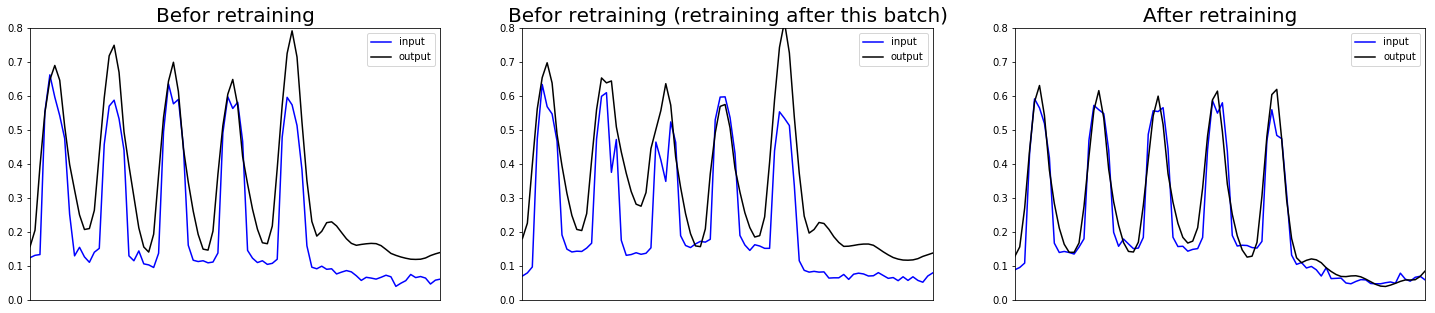
\includegraphics[width=15cm, height=4cm]{power_retraining}
\caption[Retraining effect on Power Demand dataset]{Retraining effect on Power Demand dataset}
\label{fig:power_retraining}
\end{figure}

During the online phase, the model is retrained two times, before batch No.10 and No. 27. After retraining, the normal data reconstruction error becomes lower while for abnormal data becomes higher, so that the classification becomes easier.

\begin{figure}[h]
\centering
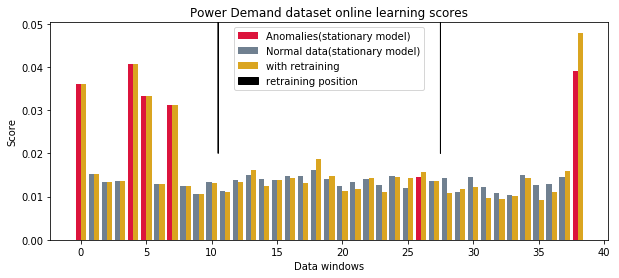
\includegraphics[width=10cm, height=4cm]{power_online_score}
\caption[Power Demand dataset online learning scores]{Power Demand dataset online learning scores}
\label{fig:power_online}
\end{figure}

After each retraining process, the parameters mu, sigma and threshold of anomaly scores are also updated. \Fref{fig:parachanges} shows the parameter changes over the stream. As there is no clear concept drift during the power demand stream, the parameters changes just slightly, and learn latest knowledge from the retrain buffer. 

\begin{figure}[h]
\centering
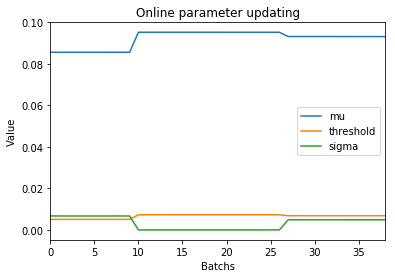
\includegraphics[width=6cm, height=4cm]{para_update}
\caption[Online parameter updating]{Online parameter updating}
\label{fig:parachanges}
\end{figure}

During the online phase, each normal window that is not given with a low enough anomaly score is appended to the retaining buffer to accumulate the retaining set. In order to find out what kind of data is used for retaining and how much retraining data is enough for model updating, we experiment with different retraining buffer size on the power demand stream.




\section{Model retraining}
\label{sec:retraining}

\subsection{Reaction of sudden and drastic concept drift}
\label{sec:reaction}
The main advantage of online model is its ability to take reaction against sudden data distributional changes in time. The SMTP+HTTP data set is composed by directly connect HTTP set after SMTP, so there is a sudden concept drift in between. The model is initialized with only SMTP data, so HTTP is completely unknown knowledge for the model. \Fref{fig:smtp+http} is a box plot of anomaly scores of normal instances from different part of the stream. The block B1 is  statistic of normal instances’ anomaly scores between the last model updating on the SMTP side and the concept drift happening, which is relative lower due to the good grasp of SMTP data. Once the concept drift takes place, namely, HTTP data arrives with the stream, more normal instances with higher anomaly score appears in B2. Although a retraining process is triggered soon after the concept drift, the normal instances’ anomaly scores still increase due to lack of HTTP instance. Gradually, with the increasing amount seen HTTP data, the model gives normal data lower anomaly score again during B4 to B6. As a result, we can observe that, when a sudden concept drift happened in the stream, our model needs only 3 to 4 times retraining with totally 3500 instances for retraining to master the new data distribution again.

\begin{figure}[h]
\centering
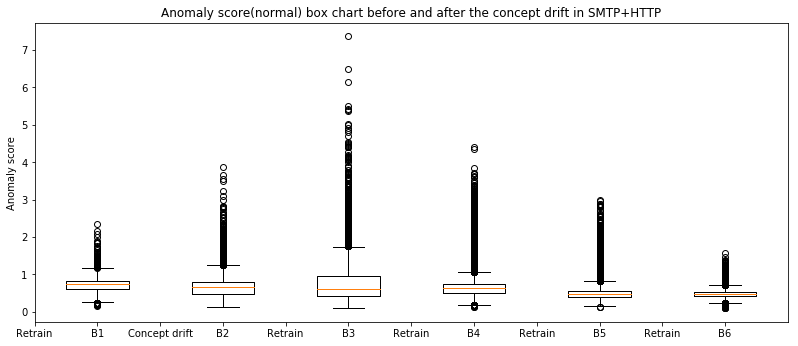
\includegraphics[width=13cm, height=6cm]{smtp+http}
\caption[Anomaly score box chart of SMTP+HTTP]{Anomaly score box chart of SMTP+HTTP}
\label{fig:smtp+http}
\end{figure}

\subsection{Reaction of serried and slight concept drift}
\label{sec:reaction}

Sometimes concept drift over the stream are slight, periodically, and potentially repeated. A single slight concept drift may not be able to trigger the retraining, but new knowledge should be save to retraining buffer, so that once the model retrained with the fresh knowledge, the model should perform well when the same concept drift happens. We experiment with the FOREST dataset. There are 7 kinds of forest cover types as labels. We take the least type No.4 as anomaly while the rest 6 kinds as normal. Cover types appears alternately over the stream, so that it could be treated as slight concept drift.\\

The model is trained with hidden size 45 and window length 20. In the beginning, 3000 windows are used for initialization, and 26050 windows comes as stream.  Every normal window contains more than 10 scores over threshold is treated as hard window and appended to retraining buffer. Also, every abnormal window is saved for threshold updating.  When retrain buffer size reaches 750, a retraining process will be triggered. The model retraining is triggered 3 times over stream. 

\begin{figure}[h]
\centering
	\begin {subfigure}[t]{0.45\textwidth}
	\centering
	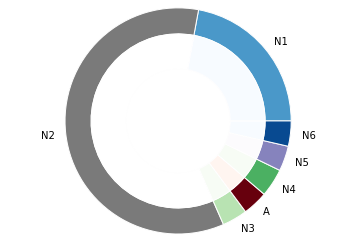
\includegraphics[height=4cm]{pie1}
	\caption{Initialization dataset}
	\label{fig:init}
	\end{subfigure}
	~
	\begin {subfigure}[t]{0.45\textwidth}
	\centering
	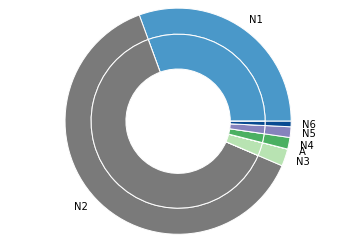
\includegraphics[height=4cm]{pie2}
	\caption{Retrain Buffer 1}
	\label{fig:buf1}
	\end{subfigure}
	~
	\begin {subfigure}[t]{0.45\textwidth}
	\centering
	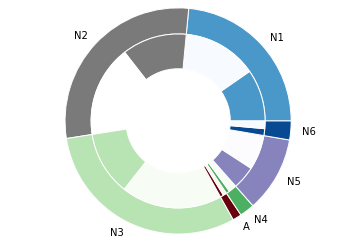
\includegraphics[ height=4cm]{pie3}
	\caption{Retrain Buffer 2}
	\label{fig:buf2}
	\end{subfigure}
	~
	\begin {subfigure}[t]{0.45\textwidth}
	\centering
	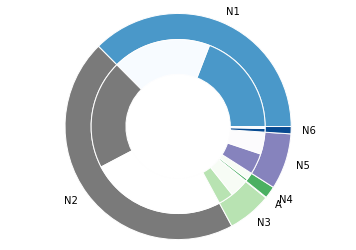
\includegraphics[height=4cm]{pie4}
	\caption{Retrain buffer 3}
	\label{fig:buf3}
	\end{subfigure}

	\caption[FOREST data initializaiton and retrain buffer data distribution]{FOREST data initializaiton and retrain buffer data distribution: N1 to N6 represent normal states from the 6 different cover type classes, and A represents anomaly, namely type4. (a) is the initialization data distribution and (b), (c), (d) are the three retrain buffers' data distribution. Outer rings are all seen data since last retraining and inner rings are the portions added to retrain buffer.}
\label{fig:bufs}
\end{figure}








